\documentclass{beamer}
\usepackage[utf8]{inputenc}


%\setbeamertemplate{headline}{}
%\setbeamertemplate{navigation symbols}{}

\def\arraystretch{1.5}%  1 is the default, change whatever you need
\newcommand*{\theorembreak}{\usebeamertemplate{theorem end}\framebreak\usebeamertemplate{theorem begin}}

\makeatletter
\newenvironment<>{proofs}[1][\proofname]{%
	\par
	\def\insertproofname{#1\@addpunct{.}}%
	\usebeamertemplate{proof begin}#2}
{\usebeamertemplate{proof end}}
\makeatother

%packages to use
%\usepackage{beamerthemesplit}
%\usepackage{verbatim}
%\usepackage{amsmath,amsfonts,amsthm,amssymb}
%\usepackage{setspace}
%\usepackage{fancyhdr}
%\usepackage{extramarks}
%%\usepackage{color}
%\usepackage{graphicx,float, wrapfig}
%\usepackage{epstopdf}
%\usepackage{transparent}
%\usepackage{eso-pic}
%\usepackage{multicol}
%\usepackage{booktabs}

%\usepackage{xcolor}
%\usepackage{cleveref}
%
%\everymath={\displaystyle}

% For mindmap
%\usepackage{dtklogos}
\usepackage{tikz}
\usetikzlibrary{mindmap,trees}


%New commands to simplify typing. You do not need to use them all, or at all.
\newcommand\Z{{\mathbb Z}}
%\newcommand{\FF}{\mathbb{F}}  \def\QQ{\mathbb{Q}} \def\R{\mathcal{R}} \newcommand{\CC}{\mathbb{C}}  \def\RR{\mathbb{R}}
%\newcommand{\Ss}{\mathbb{S}}
%\def\g{\mathfrak{g}} \def\h{\mathfrak{h}} \def\ad{\mathrm{ad}}
%\def\tr{\mathrm{tr}} \def\dim{\mathrm{dim}} \def\Hom{\mathrm{Hom}}
%\def\End{\mathrm{End}} \def\ZZ{\mathbb{Z}} \def\Aut{\mathrm{Aut}}
% \def\X{\mathfrak{X}} \def\sl{\mathfrak{sl}}\def\H{\mathcal{H}} \def\Ind{\mathrm{Ind}} \def\GL{\mathrm{GL}} \def\ind{\mathrm{ind}}  \def\Res{\mathrm{Res}} \def\dd{\displaystyle} \def\Inf{\mathrm{Inf}} \def\ch{\mathrm{ch}} \def\spanning{\textnormal{-span}}
%\def\vphi{\varphi} \def\U{\mathcal{U}} \def\P{\mathcal{P}}\def\B{\mathcal{B}}
%\def\Irr{\mathrm{Irr}} \def\veps{\varepsilon} \def\wt{\mathrm{wt}}\def\Indf{\mathrm{Indf}}
%\def\Resf{\mathrm{Resf}} \def\L{\mathcal{L}} \def\sh{\mathrm{sh}}\def\hgt{\mathrm{ht}}
%\def\diag{\mathrm{diag}} \def\Card{\mathrm{Card}} \def\scscs{\scriptscriptstyle} \def\scs{\scriptstyle}
%\newcommand{\cT}{\mathcal{T}}\newcommand{\cD}{\mathcal{D}}  \newcommand{\BC}{\mathbf{C}}
%\newcommand{\cN}{\mathcal{N}}
%\newcommand{\cX}{\mathcal{X}}
%\newcommand{\cS}{\mathcal{S}}
%\newcommand{\cB}{\mathcal{B}}
%\newcommand{\cI}{\mathcal{I}}
%\newcommand{\cC}{\mathcal{C}}
%\newcommand{\cK}{\mathcal{K}}
%\newcommand{\cM}{\mathcal{M}}
%\newcommand{\cE}{\mathcal{E}}
%\newcommand{\cQ}{\mathcal{Q}}
%\def\ts{\textstyle}
%\newcommand{\character}{\mathrm{char}}
%\newcommand{\Tr}{\mathrm{Tr}}
%\def\cP{\mathcal{P}}
%\newcommand{\cL}{\mathcal{L}}
%\newcommand{\cR}{\mathcal{R}}
%\newcommand{\cA}{\mathcal{A}}
%\newcommand{\cH}{\mathcal{H}}
%\newcommand{\One}{{1\hspace{-.14cm} 1}}
%\newcommand{\one}{{1\hspace{-.11cm} 1}}
%\newcommand{\entryr}[1]{\sss{\overrightarrow{\underset{\circ}{#1}}}}
%\newcommand{\entryl}[1]{\sss{\underleftarrow{\overset{\circ}{#1}}}}
%\newcommand{\btr}{\mathrm{btr}}
%\newcommand{\Id}{\mathrm{Id}}
%\newcommand{\im}{\mathrm{im}}
%\newcommand{\LL}{\mathrm{LL}}
%\newcommand{\RL}{\mathrm{RL}}
%\newcommand{\Sq}{\mathrm{Sq}}
%\newcommand{\supp}{\mathrm{supp\,}}
%\newcommand{\CKP}{C_{\scscs{\tiny{KP}}}}
%\newcommand{\larc}[1]{\hspace{-.4ex}\overset{#1}{\frown}\hspace{-.4ex}}
%\newcommand{\slarc}[1]{\overset{#1}{\frown}}
%\newcommand{\D}[3]{D^{#1}\left(#2,#3\right)}
%\newcommand{\Da}[3]{\tilde{D}^{#1}\left(#2,#3\right)}
%\newcommand{\hd}[3]{d^{#1}\left(#2,#3\right)}
%\newcommand{\hda}[3]{\tilde{d}^{#1}\left(#2,#3\right)}
%\newcommand{\frexp}[2]{^{\frac{#1}{#2}}}
%\newcommand{\inv}{^{-1}}
%\newcommand{\sleq}{\leqslant}
%\newcommand{\sgeq}{\geqslant}
%\newcommand{\twid}[1]{\widetilde{#1}}
%\newcommand{\meang}{\measuredangle}


%%%%%%%%%%%%%%%%%%%

% Theorem environments
\theoremstyle{definition}% default
\newtheorem{thm}{Theorem}[section]
\newtheorem{algorithm}{Algorithm}
\newtheorem{lem}[thm]{Lemma}
\newtheorem{prop}[thm]{Proposition}
\newtheorem{cor}[thm]{Corollary}
\newtheorem*{remark}{Remark}
\newtheorem{defn}[thm]{Definition}
\newtheorem{exmp}[thm]{Example}

% Information included in title page:
\usetheme{JuanLesPins}
\usecolortheme{beaver}
\title{Testing for Compositeness}
\subtitle{Miller-Rabin vs Support Vector Machine Classification}
\author{Miguel Amezola}
\institute{Department of Mathematics\\ Pacific Lutheran University}
\date{\today}
\logo{
\includegraphics[height=0.5cm]{logo}}


\AtBeginSection[]
{
	\begin{frame}
		\frametitle{Overview}
		\tableofcontents[currentsection]
	\end{frame}
}

\begin{document}

% Title page
\begin{frame}
\titlepage
\end{frame}


\section{Introduction}
\begin{frame}
	\frametitle{Prime and Composite Numbers}
	
	\begin{definition}[Prime]\label{definition:prime}
		Let $p \in \Z$, $p > 1$. Then $p$ is prime if and only if for every $a, b \in \Z$, $p=ab$ implies $a=1$ or $b=1$. \cite{pommersheim}
	\end{definition}
	
	\begin{definition}[Composite]\label{definition:composite}
		Let $n \in \Z, n > 1$. Then $n$ is composite if and only if there exists $a, b \in \Z$ such that $n=ab, 1<a,b<n$. \cite{pommersheim}
	\end{definition}		
\end{frame}


\begin{frame}
	\begin{center}

		\resizebox{!}{0.98\textheight}{%
	
			\begin{tikzpicture}
			\path[mindmap,concept color=black,text=white]
			node[concept] {Background for Miller-Rabin Test}
			[clockwise from=0]
			child[concept color=green!50!black] {
				node[concept] {Divisibility}
				[clockwise from=45]
				child { node[concept] {GCD} }
				child { node[concept] {Linear Combinations} }
			}
			child[concept color=blue] {
				node[concept](congruence) {Congruence}
				[clockwise from=30]
				child { node[concept] {Equivalent Conditions}
					[clockwise from=10]
					child { node[concept] {$\exists k \in \Z : a=b+ kn$} }
					child { node[concept] {$n \mid a - b$} }
					child { node[concept] {$a \equiv b \pmod n$} }
					}
				child { node[concept](classes) {Classes} 
					[clockwise from=-90]
					child { node[concept] {$\bar{a} = \{ x \in \Z : x \equiv a \pmod n \}$} }
					}
				child { node[concept] {Equality}
					[clockwise from=180]
					child { node[concept] {$\bar{a} = \bar{b}$ iff $a \equiv b \pmod n$} } 
				}		
			}
			child[concept color=orange] { node[concept] {Structure}
				[clockwise from=-90]
				child { node[concept] {Monoid} 
					child[grow=-45] { node[concept] {Set} }
					child[grow=-90] { node[concept] {Associative Binary Operation} }
					child[grow=-135] { node[concept] {Identity Element} }
					}
				child { node[concept] {Abelian Group} 
					child[grow=-110] { node[concept] {Monoid} }
					child[grow=-155] { node[concept] {Inverse} }
					child[grow=-200] { node[concept] {Commutative Operation} }
					}
				child { node[concept] {Ring}
					[clockwise from=-180]
					child[grow=190] { node[concept] {Disribution} }
					child[grow=140] { node[concept] {Abelian Group Under Addition} }
					child[grow=90] { node[concept] {Monoid Under Multiplication} }
					}				
			};
%			\node [annotation,right] at (classes.south)
%			{The root concept is, in general, the most important concept.};
			\end{tikzpicture}
		}
	\end{center}
			
\end{frame}

\section{Structure of $\Z_p$}
\begin{frame}
	\frametitle{Congruence Example}

	\begin{definition}[Congruent]\label{definition:congruent}
		Let $a,b,n \in \Z$ with $n > 0$. We say that $a$ is congruent to $b$ modulo $n$ if $n \mid (a - b)$, denoted $a \equiv b \pmod n$. \cite{pommersheim}
	\end{definition}
	
	\begin{example}\label{example:congruent}
		Is it true that 34 is congruent to 144 modulo $10$? Subtracting 144 from 34, we have $34 - 144 = -110$. Now, does $10$ divide this difference? Yes, since $-110 = -11 \cdot 10$. Thus, $34 \equiv 144 \pmod{10}$.
	\end{example}
\end{frame}	
\begin{frame}
	\frametitle{The Set of All Congruence Classes}
	\begin{definition}[Congruence Class]\label{definition:congruence_class}
		%		Let $n \in \N$, and let $b \in \Z$. Then the \textbf{congruence class} of $b$ modulo $n$ is the set of all integers congruent to $b$ modulo $n$: $$ \bar{b} := \{ x \in \Z : x \equiv b \pmod n \}. $$ The congruence class of $b$ modulo $n$ may also be defined as $$ \bar{b} := \{ b + kn : k \in \Z \}. $$
		Let $a,n \in \Z$ with $n > 0$. We define the congruence class of $a$ modulo $n$ as the set of all integers congruent to $a$ modulo $n$; that is, $$\bar{a} := \{ x \in \Z : x \equiv a \pmod n \}.$$% $$ \bar{a} := \{ a + kn : k \in \Z \}.$$
	\end{definition}
	
	\begin{definition}[$\Z_n$]\label{Definition: Zn}
		Let $n > 0$ be any integer. We define $\Z_n$ to be the set of all congruence classes modulo $n$, i.e. $$ \Z_n := \{ \bar{0}, \bar{1}, \bar{2}, \ldots, \overline{n - 1} \}.$$
	\end{definition}

\end{frame}


\begin{frame}
	\frametitle{The Structure of $\Z_n$}	
	
	\begin{table}[h!]
		\centering
		\begin{minipage}{0.48\textwidth}
			\centering
			\caption{Multiplication in $\Z_7$}
			\label{Multiplication in Z_7}
			\begin{tabular}{|c|c|c|c|c|c|c|c|}
				\hline
				$\cdot$		& $\bar{0}$ & $\bar{1}$ & $\bar{2}$ & $\bar{3}$ & $\bar{4}$ & $\bar{5}$ & $\bar{6}$ \\ \hline
				$\bar{0}$	& $\bar{0}$ & $\bar{0}$ & $\bar{0}$ & $\bar{0}$ & $\bar{0}$ & $\bar{0}$ & $\bar{0}$ \\ \hline
				$\bar{1}$	& $\bar{0}$ & $\bar{1}$ & $\bar{2}$ & $\bar{3}$ & $\bar{4}$ & $\bar{5}$ & $\bar{6}$ \\ \hline
				$\bar{2}$	& $\bar{0}$ & $\bar{2}$ & $\bar{4}$ & $\bar{6}$ & $\bar{1}$ & $\bar{3}$ & $\bar{5}$ \\ \hline
				$\bar{3}$	& $\bar{0}$ & $\bar{3}$ & $\bar{6}$ & $\bar{2}$ & $\bar{5}$ & $\bar{1}$ & $\bar{4}$ \\ \hline
				$\bar{4}$	& $\bar{0}$ & $\bar{4}$ & $\bar{1}$ & $\bar{5}$ & $\bar{2}$ & $\bar{6}$ & $\bar{3}$ \\ \hline
				$\bar{5}$	& $\bar{0}$ & $\bar{5}$ & $\bar{3}$ & $\bar{1}$ & $\bar{6}$ & $\bar{4}$ & $\bar{2}$ \\ \hline
				$\bar{6}$	& $\bar{0}$ & $\bar{6}$ & $\bar{5}$ & $\bar{4}$ & $\bar{3}$ & $\bar{2}$ & $\bar{1}$ \\ \hline
			\end{tabular}
		\end{minipage}
		\hfill
		\begin{minipage}{0.48\textwidth}
			\centering
			\caption{Multiplication in $\Z_8$}
			\label{Multiplication in Z_8}
			\begin{tabular}{|c|c|c|c|c|c|c|c|c|}
				\hline
				$\cdot$		& $\bar{0}$ & $\bar{1}$ & $\bar{2}$ & $\bar{3}$ & $\bar{4}$ & $\bar{5}$ & $\bar{6}$ & $\bar{7}$ \\ \hline
				$\bar{0}$	& $\bar{0}$ & $\bar{0}$ & $\bar{0}$ & $\bar{0}$ & $\bar{0}$ & $\bar{0}$ & $\bar{0}$ & $\bar{0}$ \\ \hline
				$\bar{1}$	& $\bar{0}$ & $\bar{1}$ & $\bar{2}$ & $\bar{3}$ & $\bar{4}$ & $\bar{5}$ & $\bar{6}$ & $\bar{7}$ \\ \hline
				$\bar{2}$	& $\bar{0}$ & $\bar{2}$ & $\bar{4}$ & $\bar{6}$ & $\bar{0}$ & $\bar{2}$ & $\bar{4}$ & $\bar{6}$ \\ \hline
				$\bar{3}$	& $\bar{0}$ & $\bar{3}$ & $\bar{6}$ & $\bar{1}$ & $\bar{4}$ & $\bar{7}$ & $\bar{2}$ & $\bar{5}$ \\ \hline
				$\bar{4}$	& $\bar{0}$ & $\bar{4}$ & $\bar{0}$ & $\bar{4}$ & $\bar{0}$ & $\bar{4}$ & $\bar{0}$ & $\bar{4}$ \\ \hline
				$\bar{5}$	& $\bar{0}$ & $\bar{5}$ & $\bar{2}$ & $\bar{7}$ & $\bar{4}$ & $\bar{1}$ & $\bar{6}$ & $\bar{3}$ \\ \hline
				$\bar{6}$	& $\bar{0}$ & $\bar{6}$ & $\bar{4}$ & $\bar{2}$ & $\bar{0}$ & $\bar{6}$ & $\bar{4}$ & $\bar{2}$ \\ \hline
				$\bar{7}$	& $\bar{0}$ & $\bar{7}$ & $\bar{6}$ & $\bar{5}$ & $\bar{4}$ & $\bar{3}$ & $\bar{2}$ & $\bar{1}$ \\ \hline
			\end{tabular}
		\end{minipage}
	\end{table}	
\end{frame}

\section{Miller-Rabin Test}
\begin{frame}[allowframebreaks]
	\frametitle{Fermat's Little Theorem}
	
	\begin{theorem}[Fermat's Little Theorem \cite{pommersheim}]\label{theorem:fermats_little_theorem}
		Let $p$ be prime, and let $\bar{a} \in \Z_p, \bar{a} \neq \bar{0}$. Then $$ \bar{a}^{p-1} = \bar{1}.$$
	\end{theorem}

	\begin{proofs}
		Let $p$ be prime, and let $\bar{a} \in \Z_p, \bar{a} \neq \bar{0}$.
		By \ref{lemma:unique_inverses_in_Zp}, we know that $\Z_p$ contains a unique inverse for each of its elements. 
		Furthermore, $\bar{1}^{-1} = \bar{1}$ and $\overline{p-1}^{-1} = \overline{p-1}$ by \ref{lemma:1_and_p-1_own_inverses}.
		Thus, $\bar{1} \cdot \bar{2} \cdot \bar{3} \cdots \overline{p-1} = \bar{1} \cdot \overline{p-1} = \overline{p-1}$. 
		Then 
		\begin{align*}
		(\bar{a} \cdot \bar{1})(\bar{a} \cdot \bar{2}) \cdots (\bar{a} \cdot \overline{p-1})
		&= \underbrace{\bar{a} \cdot \bar{a} \cdots \bar{a}}_{p-1 \text{ times}} \cdot \bar{1} \cdot \bar{2} \cdots \bar{a} \cdots \bar{a}^{-1} \cdots \overline{p-1} \\
		&= \bar{a}^{p-1} \cdot \overline{p-1}.
		\end{align*}
		Moreover, since this multiplication is a binary operation, we know that each product is equal to a unique element in $\Z_p$.
		Thus, $(\bar{a} \cdot \bar{1})(\bar{a} \cdot \bar{2}) \cdots (\bar{a} \cdot \overline{p-1}) = \bar{1} \cdot \bar{2} \cdots \overline{p-1}$, where the right-hand side is some permutation of the elements in $\Z_p$.
	\end{proofs}
	
	\begin{proofs}[\proofname\ (Cont.)]
		Hence,
		\begin{align*}
		\bar{a}^{p-1} \cdot \overline{p-1} 
		&= \bar{1} \cdot \bar{2} \cdots \overline{p-1} \\
		\bar{a}^{p-1} \cdot \overline{p-1}
		&= \overline{p-1} \\
		\bar{a}^{p-1}\cdot \overline{p-1} \cdot \overline{p-1}
		&= \overline{p-1}	\cdot \overline{p-1} \\
		\bar{a}^{p-1}\cdot \bar{1} 
		&= \bar{1}  \\
		\bar{a}^{p-1}
		&= \bar{1}.
		\end{align*}
		Therefore, if $p$ is prime, then $\bar{a}^{p-1} = \bar{1}$ for all $\bar{a} \in \Z_p, \bar{a} \neq \bar{0}$.
	\end{proofs}
		
\end{frame}

\begin{frame}
	\frametitle{Miller-Rabin Test for Compositeness}

	\begin{algorithm}[Miller-Rabin Test for Compositeness]\label{algorithm:miller-rabin}
		Let $n>0$ be any odd integer. 
		Then there exists an integer $k > 0$ such that $2^k$ is that largest power of two that divides $n-1$.
		If there exists $\bar{a} \in \Z_n$ such that  
		$$\bar{a}^{\frac{n-1}{2^k}} \neq \bar{1}$$ and 
		$$\bar{a}^{\frac{n-1}{2^h}} \neq -\bar{1},$$ 
		for all $h \in \Z : 1 \leq h \leq k$, then $n$ is composite. 
		In this case, the integer $a$ is called a Miller-Rabin witness to the compositeness of $n$.
	\end{algorithm}
	
\end{frame}

\begin{frame}[allowframebreaks]
	\frametitle{Miller-Rabin Test Example}
	
	\begin{example}
		We would like to test the compositeness of 169. Since $2^3$ is the largest power of two that divides 168, we must find an $\bar{a}\in \Z_{169}$ such that $\bar{a}^{\frac{168}{2^3}} \neq \bar{1}$ and $\bar{a}^{\frac{168}{2^h}} \neq -\bar{1}$ for all $h$, $h=1,2,3$. So, we randomly choose $\overline{19} \in \Z_{169}$ and find that
		\begin{align*}
		\overline{19}^{\frac{168}{2^3}} &= \overline{70} \\
		\overline{19}^{\frac{168}{2^2}} &= -\bar{1} \\
		\overline{19}^{\frac{168}{2^1}} &= \bar{1}. \\
		\end{align*}
		\theorembreak
		Because $\overline{19}^{\frac{168}{2^2}} = -\bar{1}$, we cannot conclude that $169$ is composite. So we randomly select a different $\bar{a} \in \Z_{169}$, namely $\bar{a} = \overline{145}$, and this time discover that
		\begin{align*}
		\overline{145}^{\frac{168}{2^3}} &= \overline{18} \\
		\overline{145}^{\frac{168}{2^2}} &= \overline{155} \\
		\overline{145}^{\frac{168}{2^1}} &= \overline{27}. \\
		\end{align*}
		Hence, $145$ is a Miller-Rabin witness to the compositeness of $169$ and we conclude that $169$ is not prime. 
	\end{example}
	
\end{frame}

\begin{frame}
	\frametitle{Effectiveness of the Miller-Rabin Test}
\end{frame}

%\begin{frame}
%	\frametitle{Machine Learning Algorithms}
%	
%	\begin{itemize}
%		\item Target function --- underlying function that maps inputs to outputs (if it exists)
%		\item Solution --- estimate of the target function by learning algorithm (also called the decision function in classification algorithms)
%		\item Hypothesis space --- a set or class of candidate solutions (known as hypotheses)
%		\item Learning algorithm --- uses training data to select a hypothesis 
%		\item Features --- the quantities used to describe the data
%		\item Attributes --- original quantities from data
%	\end{itemize}
%	
%\end{frame}

\section{Suppose Vector Machine}

\begin{frame}
	\frametitle{What is a Support Vector Machine (SVM)?}
	\begin{itemize}
		\item Use non-linear function $K$ to map input vector to a higher dimensional feature space 
		
		\item Linear decision function with maximal margin between vectors of different classes
	
	\end{itemize}
	
	\begin{center}
		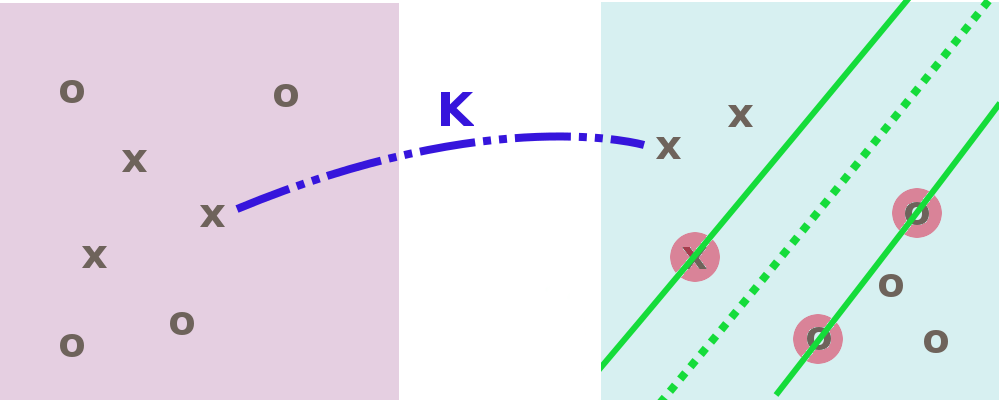
\includegraphics[width=\textwidth]{svm_graph}
	\end{center}
	
\end{frame}

\begin{frame}
	\frametitle{Linear Classification}
\end{frame}

\begin{frame}
	\frametitle{Support Vector Machine}
\end{frame}

\begin{frame}
	\frametitle{Feature Space}

	Let $b \in \Z : b \geq 2$. Then every $N \in \Z : N > 0$ can be expressed uniquely in the form $N = a_kb^k + a_{k-1}b^{b-1} + \cdots + a_1 b + a_0$, where $a_0, a_1, \ldots, a_k$ are nonnegative integers less than $b$, $a_k \neq 0$, and $k \geq 0$. \cite{koshy}

\end{frame}

\begin{frame}
	\frametitle{Training Methodology}
	
	\begin{definition}[Training Set]
		A \textbf{training set} is a collection of training examples, which are also called training data. It is usually denoted by $S = \{ (x_1, y_1),(x_2, y_2),\ldots, (x_n, y_n)\} \subset X \times Y$, where $n$ is the number of examples. We refer to $x_i$ as examples or instances and $y_i$ as their labels.\cite{christianini}
	\end{definition}
	
\end{frame}

\begin{frame}
	\frametitle{Comparison}
\end{frame}

\begin{frame}[allowframebreaks]
	\frametitle{References}
	\bibliographystyle{amsalpha}
	\bibliography{../report/refs.bib}	
\end{frame}

\begin{frame}
	\frametitle{Acknowledgements}
\end{frame}


\end{document}
